\section{Video Upload}
\label{sec:video_upload}

Upload delle video lezioni ha inizio con la selezione da parte dell’utente di un contenuto multimediale, in particolare modo il click esegue la seguente porzione di codice:
\begin{lstlisting}[language=html]
   <form class="form">
      <input-s3-video collection="videos" folder="{{folder}}"
        response="{{video}}" error="{{error}}" on-complete="on_response">
      </input-s3-video>
    </form>
\end{lstlisting}

il processo innescato può essere sintetizzato e chiarito con l’immagine seguente


\begin{figure}[htb]
 \centering
 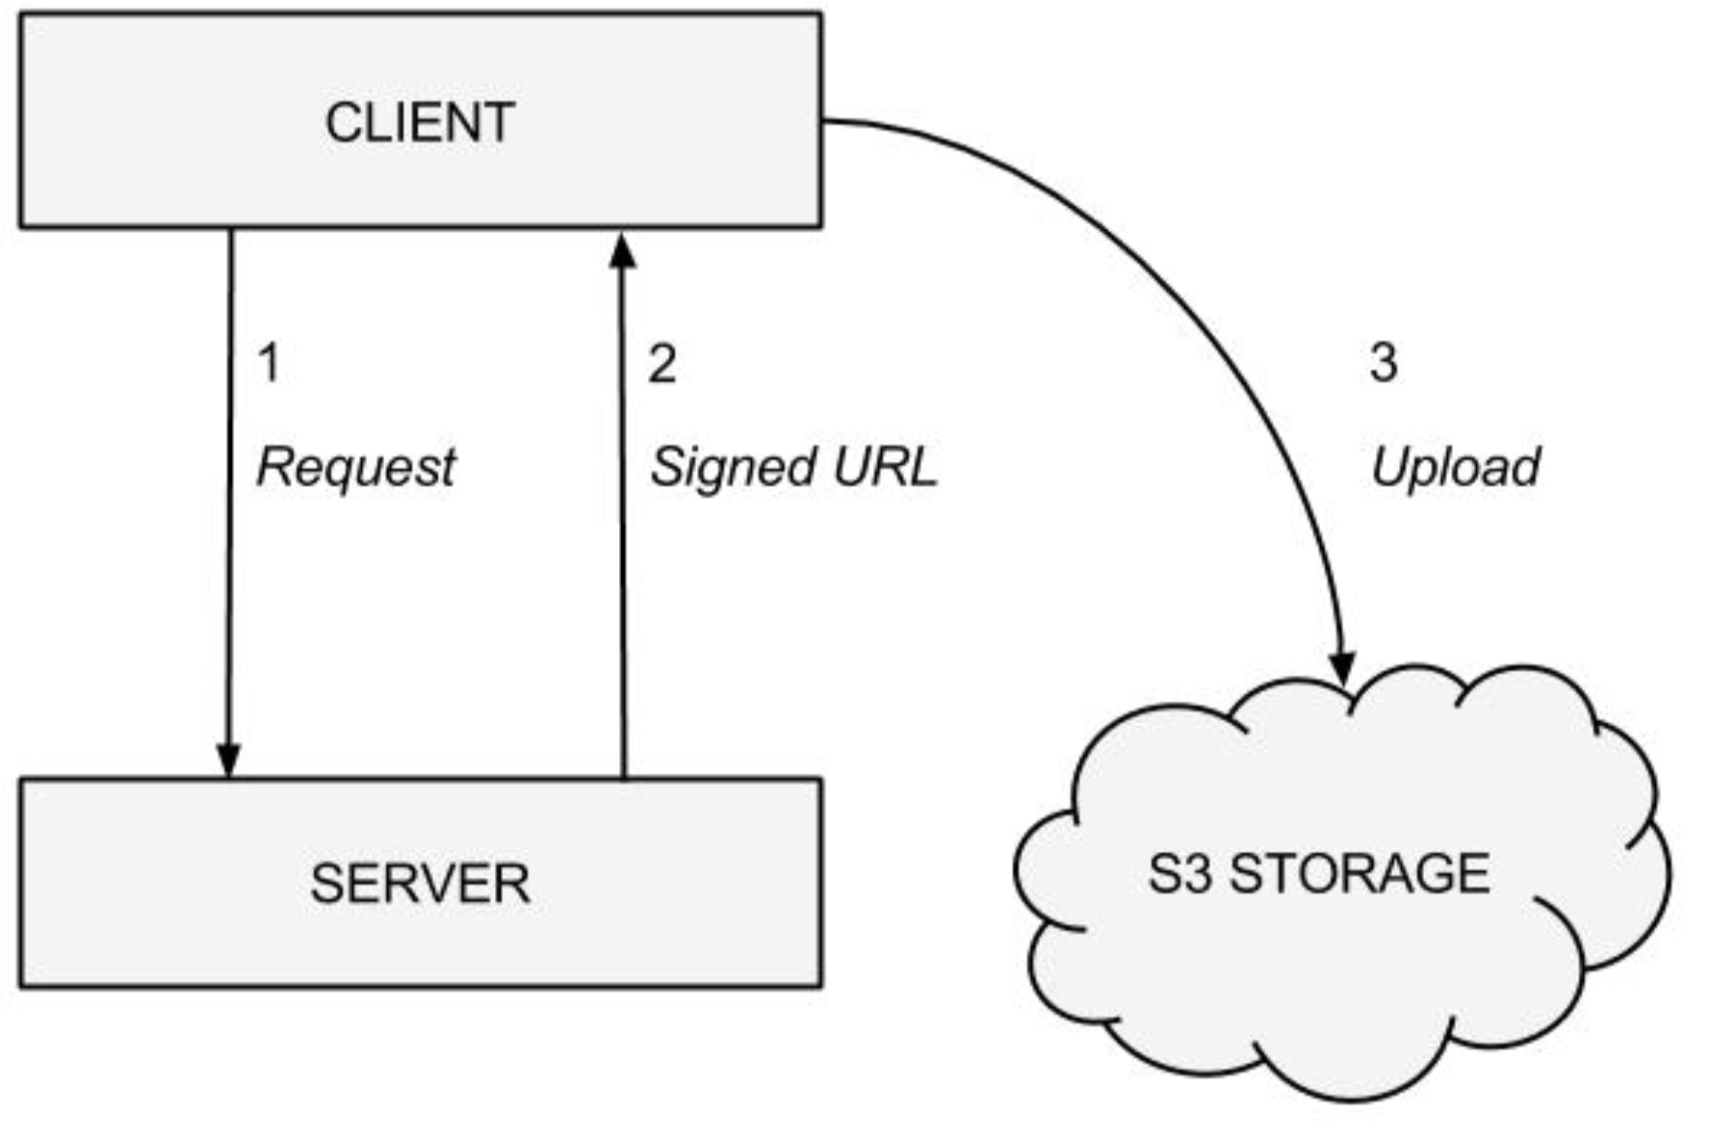
\includegraphics[width=1.0\linewidth]{images/chapter6/upload.png}\hfill
 \caption[Web Components]{Video upload}
 \label{fig:fourV}
\end{figure}




E’ possibile notare come il processo di upload si articola in tre fasi che ora andremo a descrivere nel dettaglio:
\begin{enumerate}
\item {Request}
   Nella prima fase viene instaurata la comunicazione con Amazon AWS, quindi il client esegue una GET al server
  \begin{lstlisting}[language=html]
  <iron-ajax id="createMultiPart" method="GET" url="{{url}}" params="{{params}}"
      last-response="{{response_get}}" on-response="on_response_get">
    </iron-ajax>
\end{lstlisting}
il server attraverso le API di AWS stabilisce una comunicazione e notifica l’inizio di un MultiPartUpload.
\begin{lstlisting}[language=javascript]
Video.create_multiPart_upload = function (file_name,file_type,callback){
    var s3_params = {
      Bucket: S3_BUCKET,
      Key: file_name,
      Expires: 6000,
      ContentType: file_type,
      ACL: 'public-read'      
    };
    s3.createMultipartUpload(s3_params, function(err, data) {
      if (err) {
        console.log(err, err.stack); // an error occurred
        callback(err);
        return;
      }else{
        callback(null, data);
      }
    });
  };
  
  Video.remoteMethod('create_multiPart_upload', {
    http: { verb: 'get' },
    accepts: [
      {arg: 'file_name', type: 'string'},
      {arg: 'file_type', type: 'string'}
    ],
    returns: {arg: 'dataId', type: 'string'}
  });

\end{lstlisting}
Successivamente il server si mette in attesa di una risposta che conterrà al suo interno un UploadId che verrà utilizzato nella fase successiva.
Nella seconda fase il contenuto multimediale selezionato per il caricamento viene suddiviso in chunks da 5Mb, che come vedremo a breve verrano caricati su S3.




\begin{figure}[htb]
 \centering
 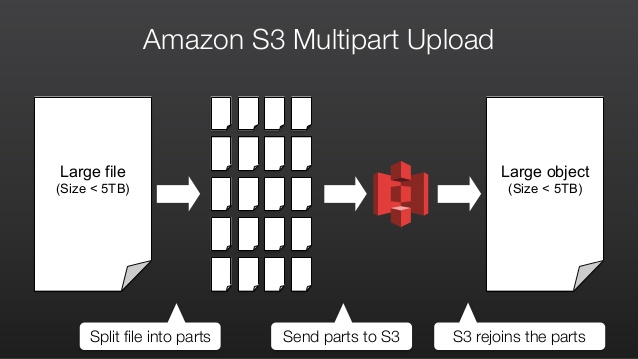
\includegraphics[width=1.0\linewidth]{images/chapter6/multipart.jpg}\hfill
 \caption[Web Components]{AWS MultipartUpload}
 \label{fig:fourV}
\end{figure}


A questo punto su ogni chunks iterativamente vengono eseguite le seguenti operazioni:



\item {Signed URL}
  * il server richiede ad AWS un Signed Url, nella richiesta tra le altre informazioni    verra inserito L’UploadId ottenuto nella fase di Request e inoltre viene specificato il     PartNumber ovvero il i-esimo chunk che sta per essere caricato.
\begin{lstlisting}[language=javascript]
  Video.signed_upload_part = function(Key,PartNumber,UploadId,callback) {
    var s3_params = {
      Bucket: S3_BUCKET,
      Key: Key,
      PartNumber: PartNumber, /* required */
      UploadId: UploadId /* required */
    };
    s3.getSignedUrl('uploadPart', s3_params, function (err, signed_url) {
      if (err) {
        console.log(err);
        callback(err);
        return;
      }
      callback(null, signed_url);
    });
  };

  Video.remoteMethod('signed_upload_part', {
    http: { verb: 'get' },
    accepts: [
      {arg: 'Key', type: 'string'},
      {arg: 'PartNumber', type: 'number'},
      {arg: 'UploadId', type: 'string'}
    ],
    returns: {arg: 'signed_url', type: 'string'}
  });
\end{lstlisting}

\item {Upload}

Nella terza e ultima fase si attende la risposta di AWS e quindi la Signed Url, che al suo interno conterrà l’ETAG, che rappresenta l’id dell’i-esimo chunk.
\begin{lstlisting}[language=html]
var ajax = document.createElement('iron-ajax');
        ajax.url = url;
        ajax.method = 'PUT';
        ajax.body = options.Body;
        ajax.handleAs='json';

        ajax.addEventListener('response', function (event) {
          var xhr = event.detail.xhr;
          var etag = xhr.getResponseHeader('ETag');
          var response = { etag: etag };
          resolve(response);
        });
\end{lstlisting}

come è possibile notare nello snippet sopra viene eseguita una PUT  contente le informazioni come ETAG e il chunk all’interno del body.
I punti 2 e 3 appena descritti vengono iterati per ogni chunk, al termine di tutti gli upload viene comunicato a S3 il termine dell’upload attraverso l’invocazione del metodo remoto seguente con il quale viene interrotta la comunicazione.

\begin{lstlisting}[language=javascript]
Video.complete_upload_part = function(Key, UploadId,Parts,callback) {
    var s3_params = {
      Bucket: S3_BUCKET,
      Key: Key,
      UploadId: UploadId,
      MultipartUpload: {
        Parts: Parts
      } 
    };
    s3.completeMultipartUpload(s3_params, function (err, signed_url) {
      if (err) {
        console.log('ERRORE COMPLETE: ' + err);
        callback(err);
        return;
      }

      callback(null, signed_url);
    });
  };

  Video.remoteMethod('complete_upload_part', {
    http: { verb: 'put' },
    accepts: [
      {arg: 'Key', type: 'string'},
      {arg: 'UploadId', type: 'string'},
      {arg: 'Parts', type: 'array' }
    ],
    returns: {arg: 'signed_url', type: 'string'}
  });
\end{lstlisting}

\end{enumerate}

